\begin{frame}{Faster R-CNN: Loss bis ep30}
\centering
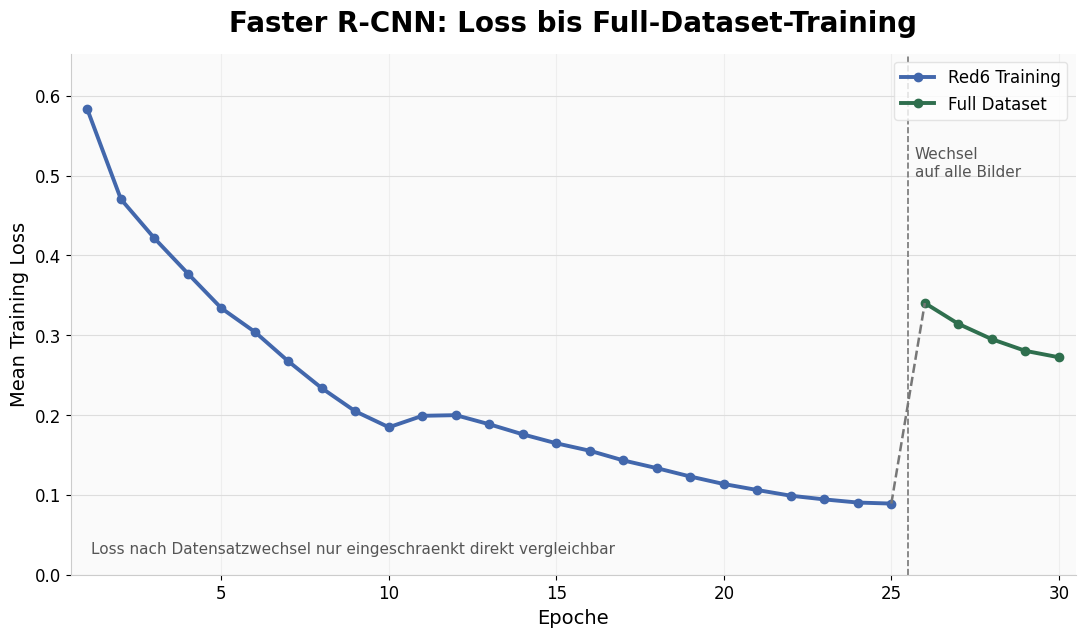
\includegraphics[width=0.92\textwidth,height=0.50\textheight,keepaspectratio]{imglib/face_model_lab/fasterrcnn_ep30_loss_entwicklung.png}

\vspace{0.2em}
\scriptsize
\begin{tabular}{l r r r}
\toprule
Trainingsphase & Bilder & Zeit & Energie (GPU, ca.) \\
\midrule
Red6 ep11--25 & 2.147 & 50,0 min & 0,08 kWh \\
Full ep26--30 & 12.880 & 74,9 min & 0,12 kWh \\
\bottomrule
\end{tabular}

\vspace{0.1em}
{\tiny Energie geschaetzt mit 100 W GPU-Mittelwert aus Faster-R-CNN-s640-Thermal-Benchmark.}
\end{frame}

\begin{frame}{Faster R-CNN: Recall bis ep30}
\centering
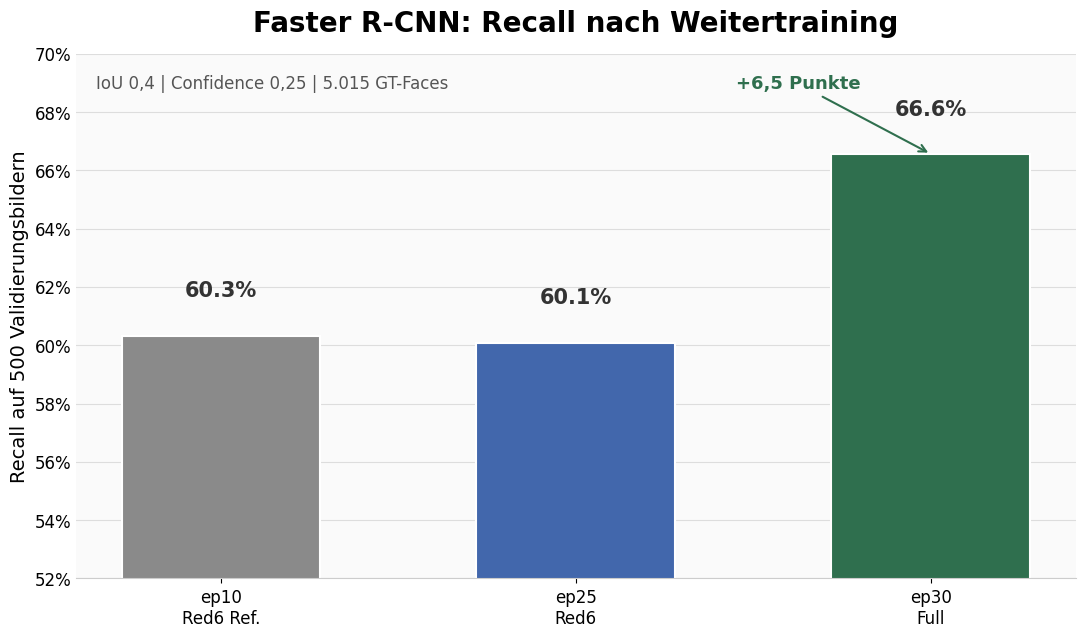
\includegraphics[width=0.92\textwidth,height=0.50\textheight,keepaspectratio]{imglib/face_model_lab/fasterrcnn_ep30_recall_vergleich.png}

\vspace{0.2em}
\scriptsize
\begin{tabular}{l r r r r}
\toprule
Modell & Eval-Bilder & GT-Faces & Recall & Inferenzzeit \\
\midrule
Red6 ep25 & 500 & 5.015 & 60,1\% & 49,5 ms/Bild \\
Full ep30 & 500 & 5.015 & 66,6\% & 49,2 ms/Bild \\
\bottomrule
\end{tabular}

\vspace{0.1em}
{\tiny Evaluation: IoU 0,4, Confidence 0,25; reine Inferenz ca. 24,7 s pro Modell.}
\end{frame}
